\documentclass[UTF8]{ctexart}
% 基本设置和必要宏包
\usepackage{geometry}
\geometry{a4paper,scale=0.8}

% 数学相关宏包
\usepackage{amsmath}
\usepackage{amssymb}
\usepackage{amsfonts}

\usepackage{mathtools}
\usepackage{amsbsy}
\usepackage{amstext}
\usepackage{wasysym}
\usepackage{stmaryrd}
\usepackage{mathrsfs}

% 图形和颜色
%\usepackage{xcolor}
\usepackage{graphicx}
\usepackage{subcaption}
\usepackage{caption}
\usepackage{float}

% 其他功能性宏包
\usepackage{titlesec}
\usepackage{fancyhdr}
\usepackage{setspace}
\usepackage{cite}
\usepackage{appendix}
\usepackage{listings}
\usepackage{pdfpages}
\usepackage{enumitem}
\usepackage{tabu}
\usepackage{threeparttable}
\usepackage{booktabs}
\usepackage{abstract}
\usepackage{multirow}


\usepackage{diagbox} 
% 设置全局字体
%\setCJKmainfont{SimSun} % 设置正文为宋体
%\setCJKsansfont{SimHei} % 设置无衬线字体为黑体

% 允许公式跨页
\allowdisplaybreaks[4]



\newcommand{\sihaoheiti}{\fontsize{14pt}\selectfont\heiti}

% 论文题目设置为三号黑体字,并居中
\newcommand{\threelargebf}{\fontsize{16pt}{19.2pt}\selectfont\heiti\centering}

% 一级标题设置为四号黑体字,并居中
\titleformat{\section}{\centering\fontsize{14pt}{16pt}\bfseries\heiti}{\thesection}{1em}{}

% 二级标题设置为小四号黑体字,左对齐
\titleformat{\subsection}{\fontsize{12pt}{14.4pt}\bfseries\heiti}{\thesubsection}{1em}{\raggedright}

% 三级标题设置为小四号黑体字,左对齐
\titleformat{\subsubsection}{\fontsize{12pt}{14.4pt}\bfseries\heiti}{\thesubsubsection}{1em}{\raggedright}

% 正文字体设置为小四号宋体字,并使用单倍行距
\renewcommand{\normalsize}{\fontsize{12pt}{14.4pt}\selectfont}


%\linespread{5.0}%修改行距
% 图片文件夹
\graphicspath{{img/}}
\let\itemize\compactitem
\let\enditemize\endcompactitem
% 设置页面布局
\geometry{a4paper, left=2.5cm, right=2.5cm, top=3cm, bottom=3cm}
\setstretch{1.2}

\renewcommand{\arraystretch}{1.5}
\newcommand{\thickhline}{\noalign{\hrule height 1.2pt}} % 设置粗线的宽度
\newcommand{\thinhline}{\noalign{\hrule height 0.8pt}} % 设置细线的宽度

%%%% ===== 定理环境
\usepackage[amsmath,thref,thmmarks,hyperref]{ntheorem} % 定理宏包
%\theorempreskipamount1em % spacing before the environment
%\theorempostskipamount0em  % spacing after the environment
%\theoremstyle{plain}
%\theoremheaderfont{\normalfont\heiti}
%\theorembodyfont{\normalfont\kaishu}
%\theoremindent0em
%\theoremseparator{\hspace{0.2em}}
%\theoremnumbering{arabic}

\newtheorem{property}{性质}[section]
\newtheorem{definition}{定义}[section]
\newtheorem{lemma}{引理}[section]
\newtheorem{remark}{注记}[section]
\newtheorem{corollary}{推论}[section]
\newtheorem{example}{例}[section] 
\newtheorem{problem}{{问题}}

 \renewcommand{\abstractnamefont}{\normalfont\bfseries}  % 摘要标题字体:正常字体,粗体
\renewcommand{\abstracttextfont}{\normalfont\normalsize}     % 摘要内容字体:正常字体,小四号

% 设置页眉页脚
\pagestyle{fancy}
\fancyhf{}
\fancyfoot[C]{\thepage}
\renewcommand{\headrulewidth}{0pt}

% 设置标题格式
\titleformat{\section}{\centering\heiti\large}{\thesection}{1em}{}
\titleformat{\subsection}{\raggedright\heiti\normalsize}{\thesubsection}{1em}{}
\titleformat{\subsubsection}{\raggedright\heiti\normalsize}{\thesubsubsection}{1em}{}

% 设置摘要环境
%\newenvironment{myabstract}{
%	\begin{center}
%	\bfseries\zihao{-3} 摘要
%	\end{center}
%	\vspace{-0.5em} % 调整摘要与论文题目的距离
%	\normalsize
%}{
%}
% 设置附录环境
\renewcommand{\appendixname}{附录}
\renewcommand{\appendixpagename}{附录}

% 设置代码环境
\lstset{
	basicstyle=\small\ttfamily,
	keywordstyle=\color{blue},
	commentstyle=\color{green!70!black},
	stringstyle=\color{red},
	breaklines=true,
	numbers=left,
	numberstyle=\tiny,
	frame=tb,
	language=Python
}
\newcommand{\bbA}{\mathbb{A}}
\newcommand{\bbB}{\mathbb{B}}
\newcommand{\bbC}{\mathbb{C}}
\newcommand{\bbD}{\mathbb{D}}
\newcommand{\bbE}{\mathbb{E}}
\newcommand{\bbF}{\mathbb{F}}
\newcommand{\bbG}{\mathbb{G}}
\newcommand{\bbH}{\mathbb{H}}
\newcommand{\bbI}{\mathbb{I}}
\newcommand{\bbJ}{\mathbb{J}}
\newcommand{\bbK}{\mathbb{K}}
\newcommand{\bbL}{\mathbb{L}}
\newcommand{\bbM}{\mathbb{M}}
\newcommand{\bbN}{\mathbb{N}}
\newcommand{\bbO}{\mathbb{O}}
\newcommand{\bbP}{\mathbb{P}}
\newcommand{\bbQ}{\mathbb{Q}}
\newcommand{\bbR}{\mathbb{R}}
\newcommand{\bbS}{\mathbb{S}}
\newcommand{\bbT}{\mathbb{T}}
\newcommand{\bbU}{\mathbb{U}}
\newcommand{\bbV}{\mathbb{V}}
\newcommand{\bbW}{\mathbb{W}}
\newcommand{\bbX}{\mathbb{X}}
\newcommand{\bbY}{\mathbb{Y}}
\newcommand{\bbZ}{\mathbb{Z}}

\title{}
\author{}
\date{}

\begin{document}


\begin{titlepage}		
		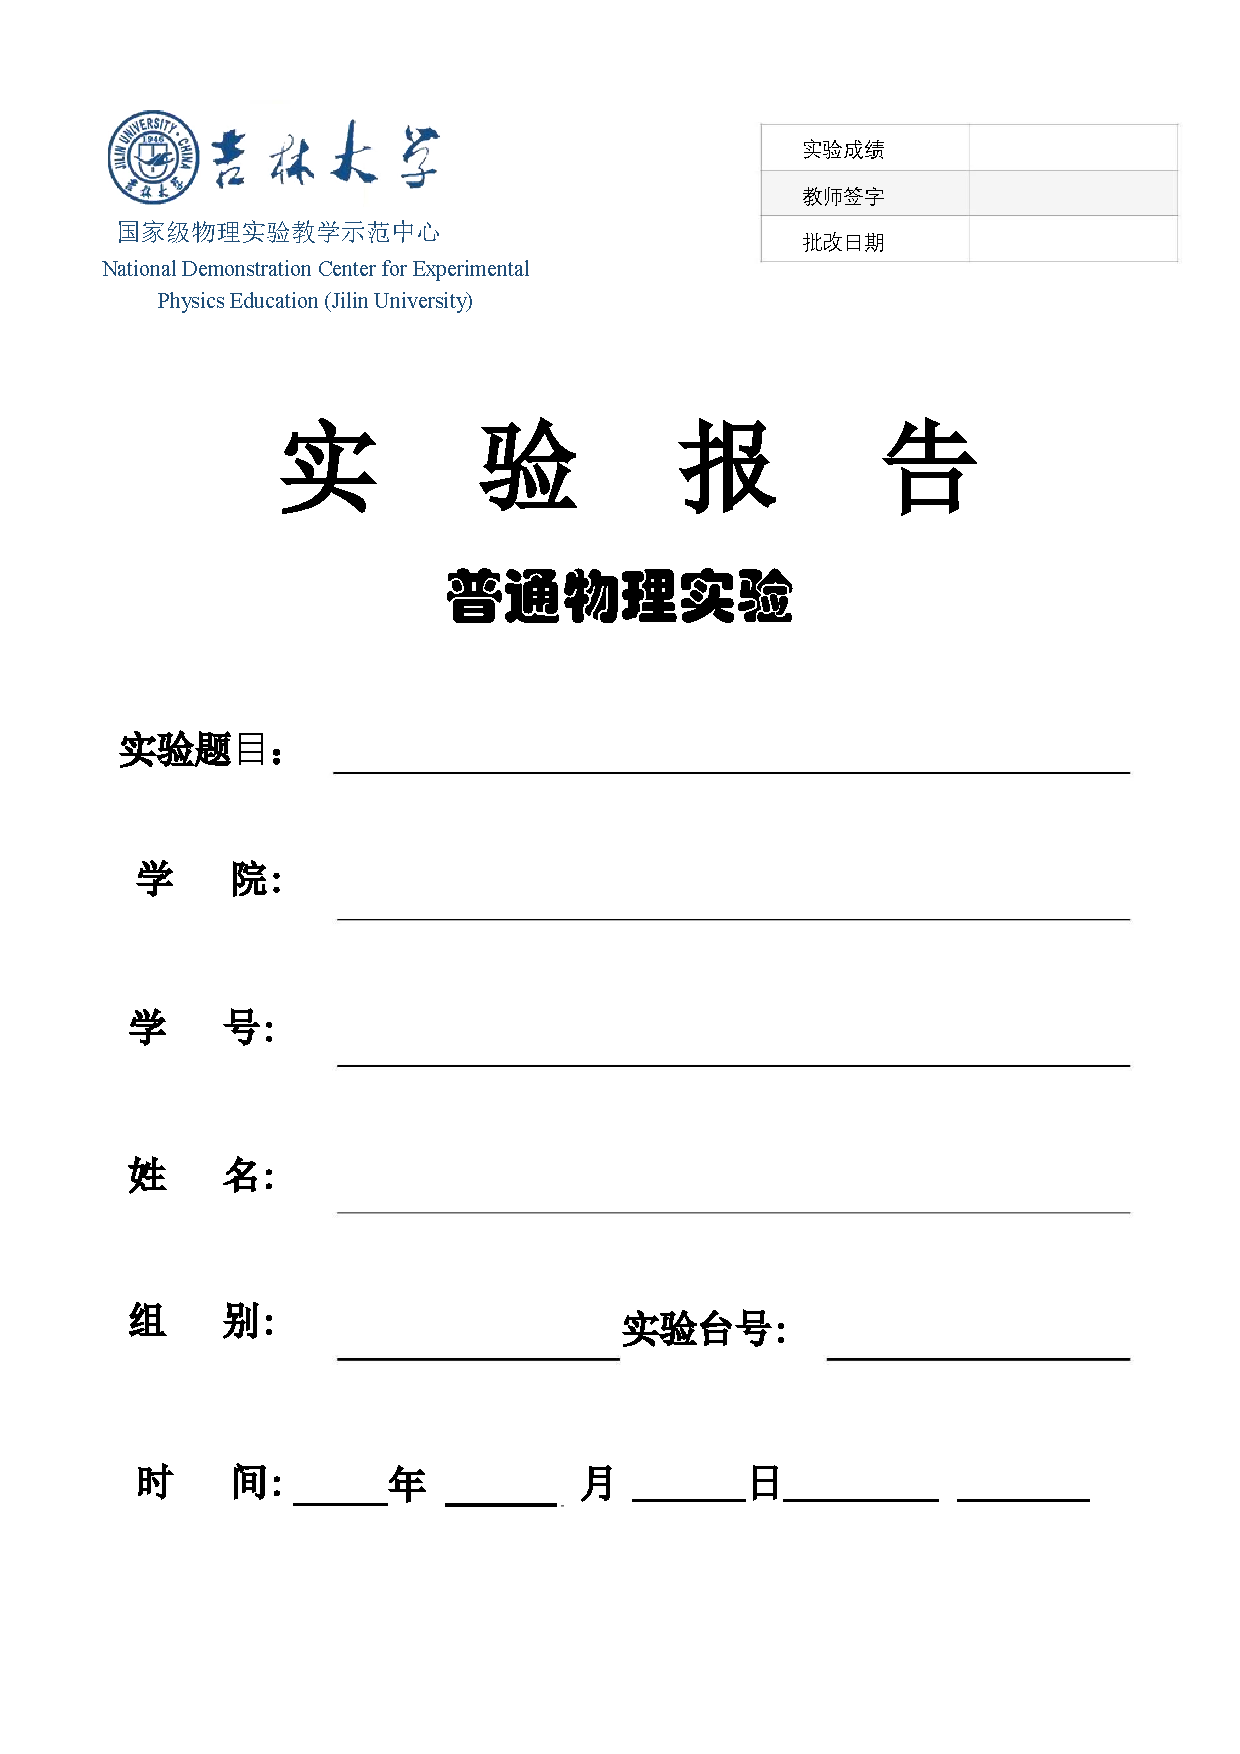
\includepdf[pages=-]{封面.pdf}
\end{titlepage}



\section{实验内容}
\begin{enumerate}
    \item 组装一个 $R_{\text{中}} = 1200 \  \Omega$ 的电阻表,对表盘进行标定并测量其电阻
    \item 用电阻箱作标准电阻对电阻表的表盘进行标定,标定至少九个点
    \item 用自制的电阻表测量三个电阻的阻值,并与指针万用表和数字万用表测得的结果进行比较
    \item 测量电路如图所示,滑线变阻器的滑键调至中心位置,分别取 $R_1 = 100 \  \Omega$、$R_2 = 200 \ \Omega$,$R_1 = R_2 = 20 k \ \Omega$ 两组数据,用指针万用表和数字万用表测量 $U_{R_1}$、$U_{R_2}$、$U_{AC}$、$U_{CB}$、$U_{AB}$
    \item 测量电路如图,取 $R_1 = R_2 = 150 \ \Omega$,用指针万用表不同量程和数字万用表电流档分别测量 $I_1$、$I_2$、$I$的值
    
\end{enumerate}
\vspace{5cm}
% 绘制书上的电路图

\section{原始数据}

\begin{table}[H]
    \centering
    \caption{标定}
    \begin{tabular}{|c|c|c|c|c|c|c|c|c|}
    \hline
       $I/mA$  & 0.9 & 0.8 & 0.7 & 0.6 & 0.5 & 0.4 & 0.3 & 0.2  \\
    \hline
        $R_x/\Omega$   &  116.6 & 283.1  & 484.2  & 794.3  & 1174.7  & 1787.5  & 2713.2 & 4742.5 \\
    \hline
    \end{tabular}
\end{table}

\begin{table}[H]
    \centering
    \caption{比较不同表的测试结果}
    \begin{tabular}{|c|c|c|c|}
    \hline
      电阻$R$ &  $R_1$   &  $R_2$  &  $R_3$  \\
     \hline
     自制电阻表电流  &  $0.731\ mA$  & $0.372\ mA$  & $0.329\ mA$ \\
     \hline
     自制电阻表   & $425 \ \Omega$  & $1984 \ \Omega$ &  $2401 \ \Omega$ \\
     \hline
     指针万用表  &  $400 \ \Omega$  &  $1900\ \Omega$  & $2380\ \Omega$  \\
     \hline
     数字万用表  &  $422\ \Omega$  & $1982\ \Omega$  &  $2404\ \Omega$  \\
     \hline
    \end{tabular}
\end{table}


\begin{table}[H]
    \centering
    \caption{万用表电压档的使用}
    \begin{tabular}{|c|c|c|c|c|c|c|c|}
    \hline
    电阻值 $R_1$、$R_2$  &  表  &  $U_{R_1}$ & $U_{R_2}$ & $U_{AC}/V$  & 
       $U_{CB}/V$    & $U_{AB}/V$  \\
    \hline
       \multirow{2}*{$R_1 = 100.0 \ \Omega,R_2 = 200.0 \ \Omega$} & 指针式 & $0.18\ V$ & $0.36\ V$ & $0.57$  & $0.85$  & $ 1.40$ \\
       & 数字 & $181.0\ mV$  &  $ 355.3\  mV$  & $0.536$  & $0.873$ & $ 1.410$ \\
    \hline
       \multirow{2}{*}{$R_1 = R_2 = 20k \ \Omega$} & 指针式 & $0.252\ V$ & $0.252\ V$ & $0.65$  & $0.749$  & $ 1.39$ \\
       & 数字 & $324.0\ mV$  &  $ 324.0\  mV$  & $0.648 $& $0.761$ & $ 1.410$ \\
    \hline
    \end{tabular}
\end{table}


\begin{table}[H]
    \centering
    \caption{万用表电流档的使用$(R_1 = R_2 = 150 \ \Omega)$}
    \begin{tabular}{|c|c|c|c|}
    \hline
         表  &  $I_1 / mA$  &  $ I_2 / mA $  &  $I/mA$  \\
    \hline
         指针式$5mA$ &   1.71   & 4.47  &  超出量程  \\
    \hline
         指针式$50mA$ &  1.7  &  4.5   &  6.2   \\
    \hline
         数字   &    1.78   &   4.57   &  6.34  \\
    \hline
    \end{tabular}
\end{table}




\section{数据处理及分析}

\subsection{电阻表的设计过程和各参量的值}
用数字万用表和指针式万用表测得电源电动势$\epsilon$均为$1.414V$,同时测得电流表内阻为 $205.2\ \Omega$,此时由于组装中值电阻$R_{\text{中}} = 1200 \ \Omega$,故电路图如图所示
\begin{align*}
    I_0 &= \frac{\epsilon}{R_{\text{中}}}  = \frac{1.414}{1200} \ A = 1.18 \  mA \\
    R_0(I_g - I_0)& = R_0 I_0\\
   \text{得} \  R_0 &= \frac{R_gI_g}{I_0 - I_g} = \frac{205.2 \times 1}{1.18-1} \  \Omega = 1150.9 \ \Omega
\end{align*}
得到$R_0 = 1150.9 \ \Omega$此时 $R_x = 0 \ \Omega$,同时
$$R_3 =  R_{\text{中}} - \frac{R_0R_g}{R_0 + R_g} = 1200 - \frac{1150.9 \times 205.2}{1150.9  + 205.2} \  \Omega =  1025.9 \ \Omega $$
计算得 $R_0 = $,$R_3 = $
按照图中图连接电路图,并测得当按指定$R_x = 0$,$R_3 = 1025.9 \ 
\Omega$连接电路时表头指针恰好满偏,故由此判定在一定程度上其表的内阻恰为 $1200 \ \Omega$

此时若电池电动势变化范围为 $\epsilon \in [1.3\ V ,1.6\ V]$

同上计算得到 当 电动势$\epsilon = 1.3 \ V$时,$R_0 = 2462.4 \ \Omega$,$R_3 = 1010.6 \ \Omega$
;当 电动势$\epsilon = 1.6 \ V$时,$R_0 = 615.6 \ \Omega$,$R_3 = 1046.1 \ \Omega$

故其变化范围为 $R_0 \in [615.6 \ \Omega, 2462.4 \ \Omega]$,$R_3 \in [ 1010.6 \ \Omega, 1046.1 \ \Omega]$


\newpage

\subsection{标定曲线}
对于上述原始数据中标定数据,使用$MATLAB$ 进行曲线拟合
\begin{figure}[H]  %h此处,t页顶,b页底,p独立一页,浮动体出现的位置
		\centering
		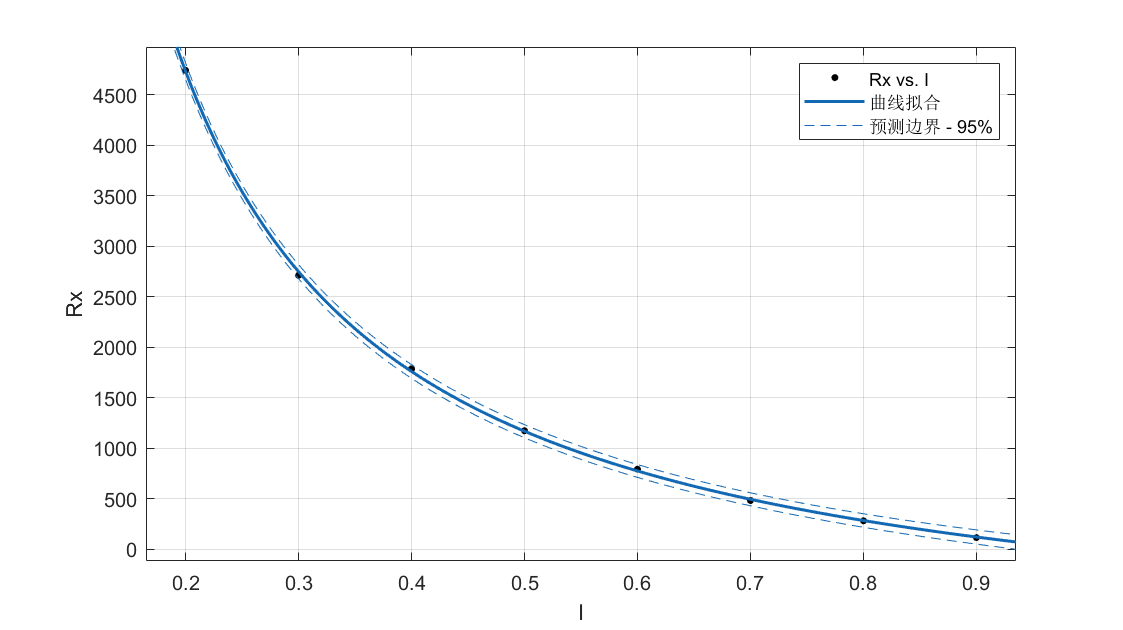
\includegraphics[width=0.8\textwidth,height=0.5\textwidth]{img/万用表拟合图像.png}
		%\caption{}
		\label{fig:side:b} 
\end{figure}
\begin{table}[H]
    \centering
    \caption*{拟合曲线$f(x) = a/x^b+c$系数和 95\% 置信边界}
    \begin{tabular}{|c|c|c|c|}
    \toprule
             &    值    &        下限       &    上限     \\
    \midrule      
a   &  1.1615e+03  &   998.1996   &    1.3248e+03       \\
    \midrule
b   &  1.0101      &   0.9411     &    1.0791           \\
    \midrule
c   & -1.1692e+03  &  -1.3714e+03 &  -966.9999  \\
    \bottomrule
    \end{tabular}
\end{table}
其中拟合优度为 $R\  \text{方} =       0.9998 ,        \text{调整} \ R \  \text{方}    = 0.9998$,拟合曲线可视为充分接近      

\subsection{用电阻箱做标准电阻标定表盘}
标定时电流的测量值和理论值存在一定的误差
\begin{enumerate}
    \item 电流计每个刻度之间差距为$0.04mA$,若指针在两个刻度线中间,则肉眼难以读出具体数值,造成读数误差
    \item 将$R_0$和$R_3$接入按理论值接入电路后,电流计恰好满偏,此时将$R_x =1200 \ \Omega$ 接入电路恰好半偏便直接进行后续操作与计算,没有对 $R_3$ 以及 $R_0$ 做微小扰动进行检验,造成微小误差。 
\end{enumerate}




\subsection{用自制电表测三个电阻并与指针式、数字万用表测量结果进行比较}
\begin{table}[H]
    \centering
    \caption*{比较不同表的测试结果}
    \begin{tabular}{|c|c|c|c|}
    \hline
      电阻$R$ &  $R_1$   &  $R_2$  &  $R_3$  \\
     \hline
     自制电阻表电流  &  $0.731\ mA$  & $0.372\ mA$  & $0.329\ mA$ \\
     \hline
     自制电阻表   & $425 \ \Omega$  & $1984 \ \Omega$ &  $2401 \ \Omega$ \\
     \hline
     指针万用表  &  $400 \ \Omega$  &  $1900\ \Omega$  & $2380\ \Omega$  \\
     \hline
     数字万用表  &  $422\ \Omega$  & $1982\ \Omega$  &  $2404\ \Omega$  \\
     \hline
    \end{tabular}
\end{table}
\begin{enumerate}
    \item 测量结果中,数字万用表电阻档的测量结果最为精确,测得结果稳定时读数,确保了读数不随电路稳定状态而发生变化
    \item 指针式万用表电阻档的测量结果需要估读,故存在一定的读数误差
    \item 自制电阻表在标定时存在一定的误差,且标定样本数较小,故拟合曲线与真实的$I-R$ 曲线存在一定的误差
    \item 经过上述分析,三者精确度:自制电阻表 $<$ 指针式万用表(电阻档) $<$ 数字万用表(电阻档)
\end{enumerate}



\subsection{万用表电压档分析仪表接入误差的影响}
\begin{table}[H]
    \centering
    \caption*{万用表电压档的使用}
    \begin{tabular}{|c|c|c|c|c|c|c|c|}
    \hline
    电阻值 $R_1$、$R_2$  &  表  &  $U_{R_1}$ & $U_{R_2}$ & $U_{AC}/V$  & 
       $U_{CB}/V$    & $U_{AB}/V$  \\
    \hline
       \multirow{2}*{$R_1 = 100.0 \ \Omega,R_2 = 200.0 \ \Omega$} & 指针式 & $0.18\ V$ & $0.36\ V$ & $0.57$  & $0.85$  & $ 1.40$ \\
       & 数字 & $181.0\ mV$  &  $ 355.3\  mV$  & $0.536$  & $0.873$ & $ 1.410$ \\
    \hline
       \multirow{2}{*}{$R_1 = R_2 = 20k \ \Omega$} & 指针式 & $0.252\ V$ & $0.252\ V$ & $0.65$  & $0.749$  & $ 1.39$ \\
       & 数字 & $324.0\ mV$  &  $ 324.0\  mV$  & $0.648 $& $0.761$ & $ 1.410$ \\
    \hline
    \end{tabular}
\end{table}
经过网络搜索可知,指针式万用表电压档内阻为$10k\ \Omega$数量级,而数字万用表电压档的内阻为$10M\ \Omega$ 
\begin{enumerate}
    \item 当 $R_1 = 100 \ \Omega$,$R_2 = 200 \ \Omega$ 时,其串联构成的电阻远小于两电表的电阻,故电表的分流可以忽略不计,故 $U_{R_1} = \frac{1}{2}U_{R_2}$,$U_{R_1} + U_{R_2} \approx U_{AC}$
    \item 当 $R_{1} = R_2 = 20k \ \Omega$,指针式万用表的内阻与电阻$R_1$、$R_2$的差别不大,其分流不能忽略,当$R_1$、$R_2$与指针式万用表并联时测得$R_1$、$R_2$两端电压明显降低,$U_{R_1} + U_{R_2} < U_{AC}$;数字式电压表内阻仍然远大于 $R_1 + R_2 = 40k \ \Omega$,从而 $U_{R_1} + U_{R_2} = U_{AC}$。
\end{enumerate}


\subsection{分析电流表内阻对测量结果的影响}

\begin{table}[H]
    \centering
    \caption*{万用表电流档的使用$(R_1 = R_2 = 150 \ \Omega)$}
    \begin{tabular}{|c|c|c|c|}
    \hline
         表  &  $I_1 / mA$  &  $ I_2 / mA $  &  $I/mA$  \\
    \hline
         指针式$5mA$ &   1.71   & 4.47  &  超出量程  \\
    \hline
         指针式$50mA$ &  1.7  &  4.5   &  6.2   \\
    \hline
         数字   &    1.78   &   4.57   &  6.34  \\
    \hline
    \end{tabular}
\end{table}


查找得指针式万用表电流档量程为$5mA$阻值约为$25 \ \Omega$,量程为$5mA$阻值约为$2.5 \ \Omega$。当电流表接入电路时,此时测 $I_1$时,即实际作用为增大了 $R_1 + R_2$的阻值。实验中滑动变阻器中值电阻远大于$R_1 + R_2 = 200 \ \Omega$,则改变 接入电路时,整体电阻减小,从而导致电流增大,而测得分路$I_1$减小;而测$I_2$接入电路时 相当于增大了 中值电阻阻值,从而与上述过程相反,增大了$I_2$的测量值;测量干路电流$I$时,等价于整个电路整体阻值变大,而导致测得电流变小。综上电流表内阻测量结果小于实际值。






















\section{思考题}

\subsection{使用指针式万用表测电阻的注意事项;如何正确选择电阻表量程和记录测量结果的有效数字}
注意事项
\begin{enumerate}
    \item 更换档位时重新调零
    \item 选择适当的量程使测量电阻时,指针尽可能指向表盘的中央位置
    \item 试验台上其余物体避免与被测量元件有接触,以免引入其余电阻
\end{enumerate}
正确选择电阻表量程

测量时应尽可能使指针指向表盘中央位置,使测量结果更加准确

正确记录测量结果的有效数字

应当读到表盘记录的最小分度值的下一位,若最小分度值以5结尾,则读到同一位


\subsection{判断电源电压下降时中值电阻的变化}
当电源电压从$1.414\ V$ 下降到 $1.3 \ V$时中值电阻发生了变化。当电动势$\epsilon$下降时,表头指针不满偏,此时需要增大 $R_0$使电流表分压增加,从而使指针满偏。故中值电阻增大

\subsection{不能用电阻表测电源内阻或灵敏电流计内阻的原因}
若用电阻表测量电源内阻,则会使电阻表和电源同时产生电动势,从而使内部电源的测量收到干扰

若使用电阻表测量灵敏电流计内阻,则电阻表调整测量量程选择超出范围时可能容易超出电流计量程,从而烧坏电流计
\subsection{判断能否用电阻表检测电容的好坏以及检测方法}
可以检测,在电阻表接到电容两端后,若指针右偏后又左偏并最后停留在$\infty$处则说明电容是好的,否则电容已经损坏

\subsection{判断改变$R_3$大小能否补偿电动势下降的变化,以及实际使用过程中采用改变并联电阻$R_0$补偿电源电动势变化的原因}
改变$R_3$大小能补偿电动势下降的变化,因为当电源电动势下降时表头指针不满偏,若此时减小$R_3$阻值,则会使表头分压增大,从而满偏

电阻$R_0$的变化和指针的偏转是同步变化的,同时由于并联表头,故改变其值对中值电阻的影响较小







\end{document}